\documentclass{article}

\usepackage[a4paper,left=18mm,right=18mm,top=20mm,bottom=18mm]{geometry}
\usepackage[italian]{babel}

\usepackage{titling}
\usepackage{graphicx}
\usepackage{subcaption}
\usepackage{float}
\usepackage{hyperref}


\title{Breve report sui risultati ottenuti tesi}
\author{David Guzman Piedrahita and Marco Vinciguerra}
 
\begin{document}
\maketitle        
\section{Introduzione}
Per questo progetto è stata fatta una rete neurale normalizzata
che contiene i dati di Moggio che vanno dal 2014 al 2020.
Per il training sono stati usati i dati dal 2014 al 2019 e per la 
validazione tutto il 2020. 
Nella validazione è stata fatta regressione.
\section{Training}
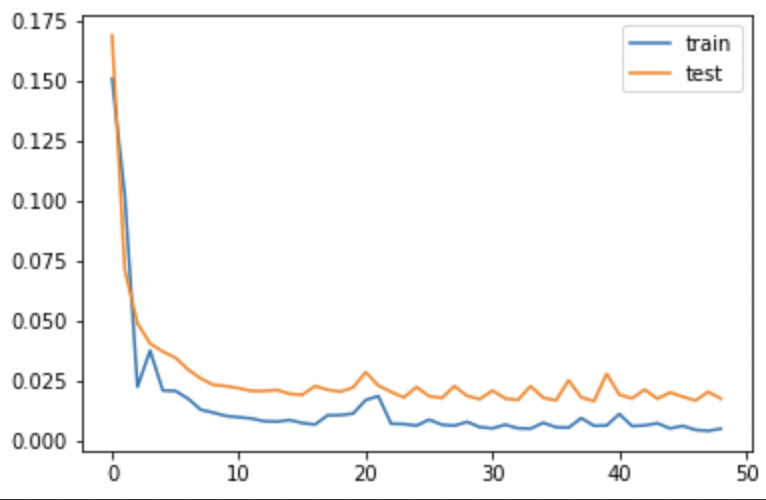
\includegraphics[scale = 0.5]{Immagini/Training.PNG}
\section{Regressione tramite reti neurali}
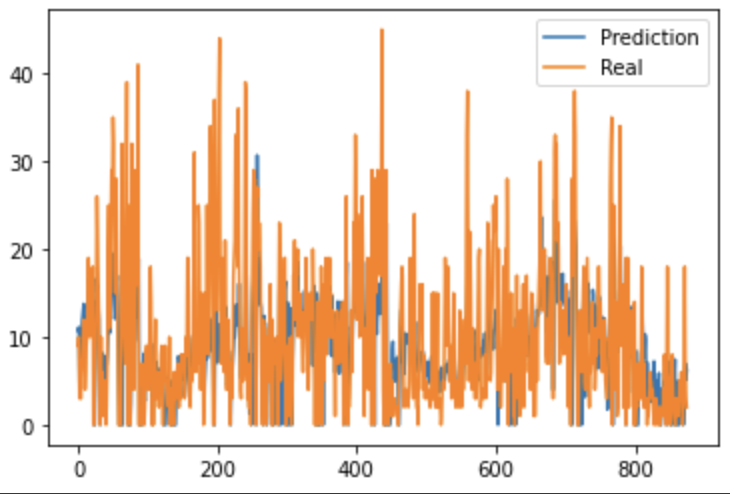
\includegraphics[scale = 0.5]{Immagini/Regressione1.PNG}
\\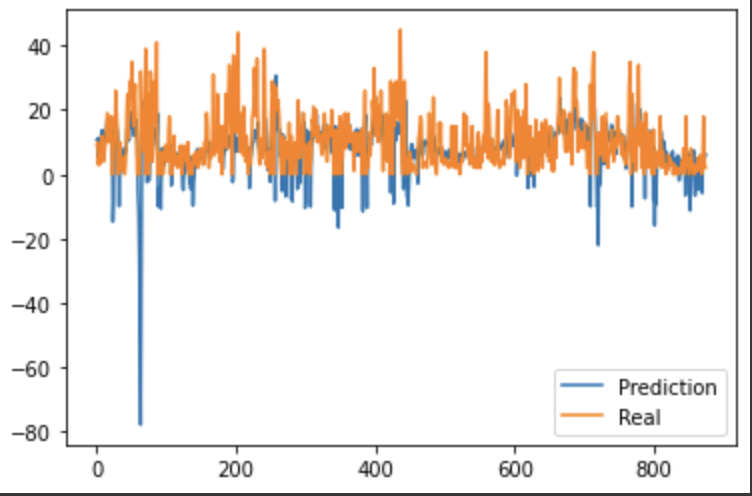
\includegraphics[scale = 0.5]{Immagini/Regressione2.PNG}
\\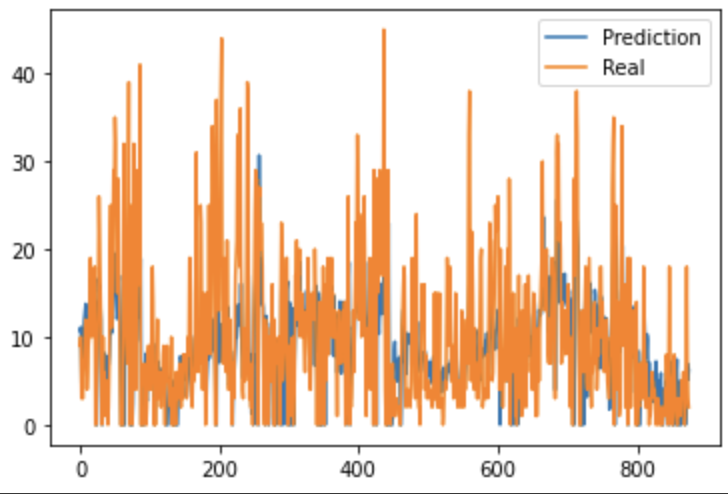
\includegraphics[scale = 0.5]{Immagini/Regressione3.PNG}
\end{document}
